
\chapter{Sistemas HAR móviles }

\label{chap4:sistemas-de-reconocimiento}

\section{Introducción}

\label{sec41:introduccion}El diseño de sistemas con conocimiento
del contexto promueven una interacción novedosa con los usuarios y
diversas aplicaciones en las áreas de ambientes inteligentes, repuesta
a emergencias, vigilancia y otros \cite{Choudhury2008}. Un sistema
con la capacidad de reconocer las actividades humanas por medio del
uso de sensores empotrados posee mecanismos para crear aplicaciones
de cuidado personal, salud y asistencia inteligente. El requerimiento
primordial de un sistema con una aplicación de contexto es que este
pueda ser portado continuamente como atuendo de sus usuarios (un sistema
\abbr{Wearable}). Por lo tanto, un sistema que acompaña continuamente
al usuario puede interaccionar oportunamente con el mismo ya que este
tiene la capacidad de observar en tiempo real las acciones de su portador.
La ventaja adicional de un sistema de este tipo es que puede ser desactivado
fácilmente o removido de la actividad diaria de su usuario.

En este capítulo se definen los componentes principales de un sistema
de reconocimiento de actividades humanas (sistemas \abbr{HAR}). El
objetivo principal del sistema \abbr{HAR} en conjunto es proveer
módulo base para aplicaciones novedosas de contexto. El módulo debe
ser capaz de reconocer varias actividades realizadas rutinariamente
de diferentes maneras, por diferentes usuarios y en diferentes condiciones
contextuales. Las funciones principales de los componentes descritos
en la primera sección exponen los mecanismos para implementar los
mismos en base trabajos relacionados de \abbr{HAR} \cite{Choudhury2008,ReyesOrtiz2015}. 

La última sección, enumera los requisitos no funcionales para lograr
una aplicación de contexto móvil y ubicua. Por un lado, las características
esperadas en una aplicación de esta naturaleza, y por el otro los
requisitos técnicos de los dispositivos móviles y los sensores empotrados
utilizados como instrumentos\footnote{\emph{hardware}} de implementación.

\section{Componentes}

\label{sec42:componentes}El diseño de la arquitectura de componentes
de un sistema \abbr{HAR} se rige de acuerdo a las guías de implementación
de una aplicación de aprendizaje automático (\abbr{ML}). De acuerdo
al proceso definido en la sección \ref{sec262:proceso-har}, se tiene
en cuenta la misma estructura de componentes y las mismas fases de
procesamiento de información. Además, se debe contemplar que el proceso
se divide en dos etapas: la etapa de entrenamiento y la de evaluación
\cite{LaraLabrador2013}. 

Ambas etapas requieren la implementación de los mismos componentes,
pero un sistema \abbr{HAR} práctico debe contemplar principalmente
la fase de evaluación, ya que el reconocimiento de actividades resulta
de una \emph{predicción} basado en un algoritmo de \abbr{ML} en-linea
(\emph{On-line learning}). Sin embargo, la etapa de entrenamiento
es un elemento clave para el sistema ya que es el punto de partida
para el \emph{aprendizaje} basado en modelo de \abbr{ML} y usualmente
se realiza bajo demanda (\emph{Off-line learning}).

Bajo el marco teórico de los sistemas \abbr{HAR} basados en \abbr{ML},
se han identificado unos componentes comunes para realizar las funcionalidades
de aprendizaje y predicción según \cite{Choudhury2008}. Un sistema
de reconocimiento de actividades posee tres componentes:
\begin{itemize}
\item un \emph{recolector }de medidas
\item un\emph{ procesador }de muestras 
\item un \emph{clasificador }de actividades
\end{itemize}
En la \figref{fig4:componentes-har} se muestra una vista general
de los componentes y sus interrelaciones. Las funcionalidades de cada
componente se describen a continuación. 

\begin{figure}[!tbph]
\centering{}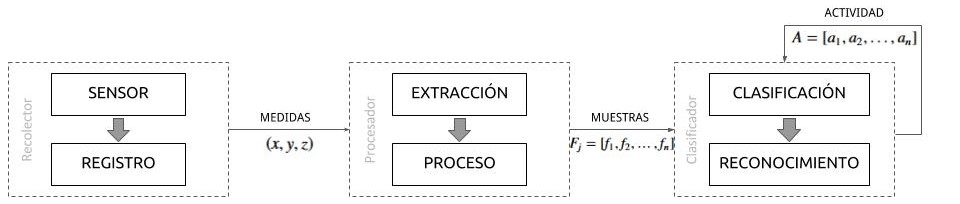
\includegraphics[width=1\linewidth]{capitulo-4/graphics/diagrama_4_1}\caption[Arquitectura de sistema HAR]{\label{fig4:componentes-har}Componentes de los sistemas \abbr{HAR}}
\end{figure}


\section{Recolector de medidas}

\label{sec43:recolector-datos}El primer paso en el proceso de reconocimiento
primeramente consiste en recolectar medidas de señales obtenidas de
los sensores que observan continuamente a los usuarios. Además, se
procede a realizar un registro de manera organizada e indexada con
respecto al tiempo. Para capturar los datos se requieren instrumentos
de medición apropiados como los sensores (\abbr{Wearables}, véase
\ref{sec23:sensores}). Los sensores capturan las señales directamente
de los usuarios por medio de observaciones continuas, al estar anexados
al cuerpo; en la cintura, la muñeca, el pectoral, los muslos o en
la cabeza \cite{Bao2004}. También, los sensores podrían ser portados
por el usuario ya están comúnmente empotrados en dispositivos de uso
regular como los teléfonos móviles modernos, en relojes o lentes inteligentes
\cite{LaraLabrador2012,Choudhury2008}.

A continuación se describe el método común de registro y organización
de los datos obtenidos de las señales continuas, además de algunos
ejemplos de variables relevantes utilizadas.

\subsection{Registro}

El método de registro consiste en capturar las señales de un sensor
y separar las medidas en una o más variables dependiendo del tipo
de sensor. La organización de los registros se realiza con respecto
al tiempo. Es decir, se dispone de un flujo continuo de datos con
una marca de tiempo almacenados de manera secuencial en un medio permanente
para su posterior procesamiento. 

La marca de tiempo usualmente se mide \emph{mili}-segundos y dependiendo
del sensor el intervalo entre medidas puede variar en el mismo orden,
Ej. con tasa de salida de \texttt{60 \abbr{Hz} }se tendrían 60 medidas
en un segundo. 

Las señales de sensores pueden clasificarse de la misma manera que
los grupos citados en la sección \ref{sec23:sensores}, según movimiento,
posición, entorno y fisiológicas. A continuación se describen en detalle
cada grupo.

\subsubsection{Señales de Movimiento}

Los sensores de movimiento proveen señales altamente informativos
para \abbr{HAR} debido a que miden las fuerzas de aceleración y rotación
en tres ejes cuando son portados por sus usuarios. En esta categoría
de sensores se encuentran los acelerómetros y giroscopios. 

Los acelerómetros miden señales de acuerdo a diferentes tipos de movimientos,
incluyendo la aceleración lineal y centrípeta, la gravedad y vibración
en dos o tres dimensiones \cite{Goehl2007}. Las variables medidas
están expresadas en la magnitud de la aceleración ejercida sobre el
dispositivo con respecto la orientación del mismo (Ej. en reposo mide
$-9.8\,m\,s^{-2}$ en dirección al suelo). La señal de la aceleración
dada por $a(t)$ es un vector con respecto al tiempo con tres componentes
en cada eje $(x,y,z)$, cada uno representa una medida $a_{x}$, $a_{y}$
y $a_{z}$. En la \figref{fig4:muestra-ac} se despliegan las medidas
obtenidas por la señal $a(t)$ durante una actividad física determinada.

\begin{figure}[!tbph]
\begin{centering}
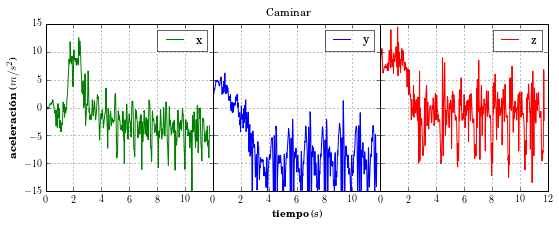
\includegraphics[width=1\columnwidth]{capitulo-4/graphics/signal_a3d}
\par\end{centering}
\caption[Señal de aceleración]{\label{fig4:muestra-ac}Señal de aceleración en tres dimensiones.
Los colores corresponden a los ejes de coordenadas representadas en
la siguiente figura.}
\end{figure}

Los giroscopios, o sensores de razón angular, miden señales de la
rapidez de rotación de los objetos en tres dimensiones \cite{Goehl2007}.
Las variables medidas están expresadas en velocidad angular de rotación
del dispositivo con respecto a los ejes de orientación del mismo (Ej.
en movimiento mide \foreignlanguage{english}{$-0.1\,rad\,s^{-1}$}
en relación a un eje fijo). La señal de la velocidad angular dada
por $w(t)$ es un vector con respecto al tiempo con tres componentes
en cada eje $(x,y,z)$, cada uno representa una medida $w_{x}$, $w_{y}$
y $w_{z}$. La orientación de los ejes con respecto al dispositivo
de medición depende del fabricante del mismo. Los teléfonos móviles
modernos poseen la orientación de los ejes de acuerdo a la siguiente
\figref{fig4:axis-phone}.

\begin{figure}[!tbph]
\begin{centering}
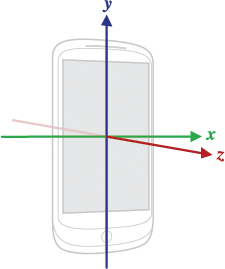
\includegraphics[scale=0.7]{capitulo-4/graphics/axis_device}
\par\end{centering}
\caption[Sistemas de coordenadas relativo a dispositivo]{\label{fig4:axis-phone}Ejes de coordenadas relativas a un teléfono
móvil moderno.}

\end{figure}

Las medidas obtenidas son variaciones con respecto a estos tres ejes
donde el valor $0$ está ubicado en el centro del dispositivo. Las
ventajas de los sensores de movimiento es su amplio uso al reconocer
actividades ambulatorias, como los citados en \cite{Bao2004,Kwapisz2011,ReyesOrtiz2015}.
Los acelerómetros y giroscopios poseen un bajo costo de fabricación,
bajo consumo de energía, y además están incluidos comúnmente en los
teléfonos móviles modernos \cite{Google2016s} debido a su utilidad
en mejorar la interacción humano-máquina por medio de gestos. Varios
trabajos publicados evidencian una alta precisión en \abbr{HAR} utilizando
al menos uno de estos sensores \cite{Bao2004,LaraLabrador2012}.

\subsubsection{Señales de Posición}

Los sensores de posición proveen señales con información adicional
que pueden ser utilizados para efectuar \abbr{HAR} y aplicaciones
de contexto con servicios basados en localización. En esta categoría
están los sensores de orientación (o brújula), magnetómetros y \abbr{GPS}
\cite{Google2016s}.

Las señales del \abbr{GPS} permiten acceder a las coordenadas geográficas
globales como el modo de transporte de un individuo, de acuerdo a
la velocidad estimada. Los teléfonos móviles modernos están equipados
con sensores para captar señales del sistema \abbr{GPS} y también
se puede estimar con buena precisión las coordenadas utilizando una
red celular \abbr{GSM}/\abbr{GPRS} y redes \abbr{WIFI} de corto
alcance. 

La señal de localización utiliza dos variables, conocidas como latitud
y longitud, y son medidas en la unidad radian (Ej. latitud $-57.2322\,rad$
y longitud $-25.3442\,rad$). Los valores de latitud y longitud son
coordenadas del \abbr{WGS} cuyos valores globales oscilan entre -180
a 180 en longitud, y -90 a 90 en latitud.

En la \figref{fig4:gps} se muestra una aplicación móvil para \abbr{Android}
que muestra el proceso de triangulación por satélites del sistema
\abbr{GPS}, donde el resultado es la estimación de las coordenadas
globales. 

\begin{figure}[!tbph]
\begin{centering}
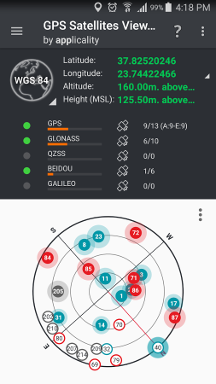
\includegraphics[scale=0.8]{capitulo-4/graphics/gps}
\par\end{centering}
\caption[Coordenadas por GPS.]{\label{fig4:gps}Visualización de satélites y coordenadas globales
basada en triagulación GPS.}
\end{figure}

Sin embargo, los \abbr{GPS} tienen cobertura limitada por la dificultad
de obtener señal dentro de edificaciones, o si no está disponible
servicio de red celular o \abbr{WIFI}. También el alto consumo de
energía es un factor importante si las aplicaciones rastrean la localización
en tiempo real. Además, la ubicación de un individuo es particularmente
información sensible para la mayoría de los usuarios y se debe tener
especial atención a no comprometer la privacidad de los datos y tener
el consentimiento del usuario para que este pueda ser rastreado \cite{LaraLabrador2013}.

\subsubsection{Señales del Ambiente}

Los sensores de ambiente miden varios atributos del entorno que rodea
al usuario. Algunas señales como la temperatura del aire, presión
atmosférica, iluminación, humedad, y el ruido pueden proveer información
de utilidad para conocer mejor el habitad particular de un usuario.
En esta categoría están los barómetros, fotómetros, termómetros y
micrófonos.

Los sensores de ambiente solos no proveen información suficiente ya
que los individuos pueden realizar las actividades bajo diversas circunstancias
contextuales en términos de clima, ruido o iluminación. Por lo tanto
estos sensores pueden utilizarse de manera complementaria para detectar
sugestiones adicionales, Ej. el usuario está en el exterior de acuerdo
a la luminosidad, o se encuentra descansando debido a un nivel de
sonido y luminosidad baja \cite{LaraLabrador2013}.

\subsubsection{Señales de Fisiológicas}

Los sensores fisiológicos proveen señales de signos vitales de un
individuo. La información sobre el ritmo cardíaco, tasa de respiración
y temperatura del cuerpo podrían ser combinados para enriquecer el
contexto durante el reconocimiento en ciertas aplicaciones específicas
como las orientadas a la salud \cite{LaraLabrador2013}.

\section{Procesador de muestras}

\label{sec44:proceso-se=0000F1ales}El siguiente paso en el reconocimiento
de actividades consiste en procesar las señales obtenidas por sensores
y extraer características relevantes de los datos en bruto. El modelo
de reconocimiento se construye a partir de un conjunto de muestras
etiquetadas utilizando métodos de aprendizaje automático en la etapa
de entrenamiento. Durante la etapa de evaluación las entradas con
las que un modelo construido opera son muestras no clasificadas pero
generadas con la misma técnica de muestreo utilizada durante el entrenamiento.

El procesador de muestras depende en tres tareas bien diferenciadas
que se realizan automáticamente en ambas etapas del proceso de reconocimiento,
adicionalmente se realiza una tarea manual durante la etapa de entrenamiento
llamada etiquetado. A continuación se detallan cada tarea.

\subsection{Etiquetado}

\label{ssec44:labeling}El proceso de aprendizaje automático requiere
de una cantidad moderada de datos recolectados a partir de usuarios
mientras realizan actividades humanas objetivas a nuestro estudio.
Estos datos deben ser recolectadas y etiquetados utilizando un teléfono
móvil inteligente con una aplicación diseñada para el caso. Ej. Utilizando
un teléfono con \abbr{Android} y la aplicación \emph{SensorLog} \cite{SLog2016}. 

El protocolo de recolección consiste en alistar un grupo de personas
que porten un teléfono inteligente mientras realizan con conjunto
específico de actividades y registrar datos por medio de la aplicación.
Las actividades de interés descritas en la sección \ref{sec263:actividades-humanas}
deben ser realizadas portando el teléfono en el bolsillo donde cada
individuo realiza una sesión de caminata, trote, bicicleta o conducir
un vehículo por un periodo de tiempo de 10 a 15 minutos. La recolección
de datos llevada a cabo por medio de la aplicación disponible para
la plataforma \abbr{Android} es mostrada en la \figref{fig4:sensor-log}. 

\begin{figure}[!tbph]
\begin{centering}
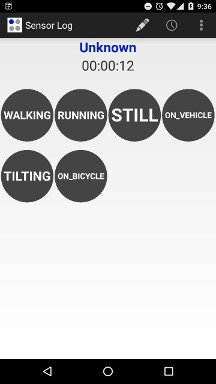
\includegraphics[scale=0.8]{capitulo-4/graphics/sensorlog1}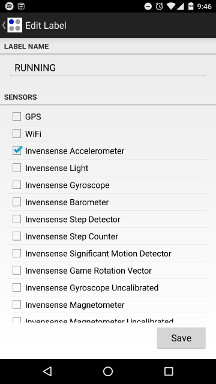
\includegraphics[scale=0.8]{capitulo-4/graphics/sensorlog2}
\par\end{centering}
\caption[Aplicación de entrenamiento SensorLog]{\label{fig4:sensor-log}Aplicación de entrenamiento \emph{SensorLog
}con interfaces de usuario para configurar y controlar la sesión de
entrenamiento}
\end{figure}

Así como se ve en la figura, la aplicación tiene una interfaz de usuario
simple que permite elegir los sensores de donde recolectar datos (Ej.
\abbr{GPS}, acelerómetro, giroscopio) para la sesión, las acciones
de iniciar y parar la actividad, y las etiquetas de la actividad que
el usuario realiza durante el entrenamiento. Las etiquetas utilizadas
en el proceso de recolección son:
\begin{itemize}
\item Caminar
\item Trotar
\item Quieto\footnote{A pesar de que esta actividad no representa un movimiento se incluye
como parte del estudio}
\item En bicicleta
\item En vehículo
\item \emph{Girando}\footnote{Esta no es una actividad física sino un comportamiento errático de
la orientación del teléfono}
\end{itemize}
La recolección se realiza obteniendo medidas a una razón de 60 a 100
\emph{mili}segundos por lo que se registran aproximadamente 60 a 100
muestras por segundo. Para asegurar la calidad de la recolección inicial
de datos las primeras sesiones de entrenamiento son supervisadas para
preparar las condiciones adecuadas del entrenamiento físico a elección
del participante.

\subsection{Filtro de Señal}

\label{ssec44:filtering}Teóricamente, si un dispositivo equipado
con sensores de movimiento está en reposo la señal de aceleración
$a(t)$ mediría cero (0) en dos ejes. Por ejemplo, en los ejes $x$
e $y$ no habría registro de medidas distintas a cero (0), y el eje
$z$mediría en dirección al suelo $-9.8\,m\,s^{-2}$. Sin embargo,
los sensores electrónicos pueden introducir cierta inestabilidad en
la señal (conocida como \emph{jitter}) provocando una fluctuación
en las lecturas debido a errores en la medición afectando la calidad
de los datos. Por lo tanto, a pesar de que un dispositivo con sensor
de movimiento esté completamente quieto en la mesa, las lecturas podrían
registrar ruido en los datos, Ej. errores del orden de $\pm0.005$. 

Entonces, para reducir ruido de la señal se debe aplicar uno o más
filtros. El filtro permite suavizar la señal por medio de una función
simple como la del cálculo de promedios variables (\emph{moving average})
o por un método como el de \emph{Butterworth} \cite{ReyesOrtiz2015}. 

Para el análisis de este trabajo se utilizó el filtro de señal de
promedios variables debido a su simplicidad y aplicabilidad basado
en otros trabajos como \cite{Yang2009}. El filtro de señal se puede
definir con la siguiente función $M$ descrita a continuación:

\label{def4:moving-average}\newtheorem{defi}{Definición}

\begin{defi}(\emph{Moving average}) Dada una secuencia $\left\{ a_{i}\right\} _{i=1}^{N}$,
un $n$-\emph{moving average} es una nueva secuencia $\left\{ s_{i}\right\} _{i=1}^{N-n+1}$
definida a partir de $a_{i}$ tomando la media aritmética de las \emph{sub}-secuencias
de tamaño $n$ donde,

\begin{eqnarray}
s_{i} & = & \frac{1}{n}\sum_{j=i}^{i+n-1}a_{j}
\end{eqnarray}

Así que las secuencias $S_{n}$ dado los $n$-\emph{moving averages}
serian 

\begin{eqnarray}
S_{2} & = & \frac{1}{2}(a_{1}+a_{2},a_{2}+a_{3},...,a_{n-1}+a_{n})
\end{eqnarray}

\begin{equation}
S_{3}=\frac{1}{3}(a_{1}+a_{2}+a_{3},a_{2}+a_{3}+a_{4},...,a_{n-2}+a_{n-1}+a_{n})
\end{equation}

y así sucesivamente.\end{defi}

Como ejemplo, en la \figref{fig4:filter-maf} se despliegan las gráficas
de una señal de aceleración $a_{y}$ para la dimensión $y$ y su correspondiente
señal filtrada con la función $M(a_{y})$ construida a partir de una
secuencia $S_{5}$ durante un intervalo de $1.6$ segundos. Como se
puede apreciar, la señal resultante está ligeramente suavizada debido
al filtrado de valores extremos resultado de perturbaciones bruscas
o ruido en la señal.

\begin{figure}[!tbph]
\begin{centering}
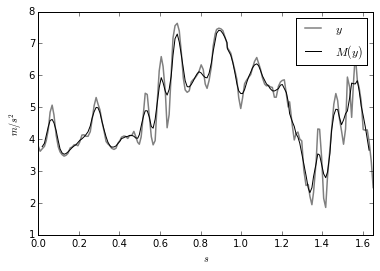
\includegraphics{capitulo-4/graphics/moving_average}
\par\end{centering}
\caption[Señal filtrada por la función $M$]{\label{fig4:filter-maf}Señal filtrada por promedios variables.}
\end{figure}


\subsection{Muestreo}

\label{ssec44:sampling}La realización de actividades humanas son
efectuadas durante periodos de tiempo de larga duración, en el orden
de los segundos o minutos. Esta taza es mucho mayor comparado con
las tazas de muestreos de los sensores, las cuales pueden llegar hasta
\texttt{250 \abbr{Hz}} (o \texttt{250} muestras por segundo). Una
simple medida capturada en un instante (Ej. la aceleración de $-2.5\,m\,s^{-2}$
en el eje $y$) no provee suficiente información para describir qué
actividad está llevando acabo un persona. Por lo tanto, las actividades
humanas deben ser reconocidas a partir de muestras extraídas en ventanas
de tiempo $w$ en vez de utilizar una sola medida instantánea en $t$. 

En la \tabref{tab4:ex-signal} se muestra una tabla con posibles medidas
instantáneas para la señal de aceleración $a(t)$ en una ventana de
tiempo $w_{j}$ con una taza de muestreo $r$asociada al sensor.

\begin{table}[!tbph]
\begin{centering}
\begin{tabular}{|c|c|c|c|c|}
\hline 
$w$ & $t$ & $a_{x}$ & $a_{y}$ & $a_{z}$\tabularnewline
\hline 
\hline 
$j$ & $0$ & \texttt{$1.3$} & \texttt{$-2.1$} & \texttt{$0$}\tabularnewline
\hline 
$j$ & $1/r$ & \texttt{$1.4$} & \texttt{$-2.3$} & \texttt{$0.1$}\tabularnewline
\hline 
$j$ & $2/r$ & \texttt{$1.1$} & \texttt{$-2.6$} & \texttt{$0$}\tabularnewline
\hline 
$j$ & $\ldots$ & \texttt{$\ldots$} & \texttt{$\ldots$} & \texttt{$\ldots$}\tabularnewline
\hline 
$j$ & $t_{max}$ & \texttt{$1.8$} & \texttt{$2.2$} & \texttt{$-0.4$}\tabularnewline
\hline 
\end{tabular}
\par\end{centering}
\caption[Medidas instantáneas de aceleración ]{\label{tab4:ex-signal}Ejemplo de medidas instantáneas de aceleración
en una ventana de tiempo.}
\end{table}

Las ventanas de tiempo hacen que las señales queden segmentadas en
muestras discretas utilizadas como unidades de reconocimiento de actividad.
De esta manera, cada ventana tiene inequívocamente una actividad humana
asociada y de esta manera podemos satisfacer el requisito planteado
por la definición del problema \ref{def2:harp-rel} en la sección
\ref{sec261:definicion-har}. 

Para incrementar la cantidad de muestras se utiliza una superposición
de $50\%$ con ventanas consecutivas y con tamaño de $2.56$ segundos,
como es recomendado por otros trabajos con técnicas de reconocimiento
\cite{Bao2004,ReyesOrtiz2015}. La superposición evita que ciertos
eventos se pierdan y las actividades se trunquen. La elección de este
tamaño de ventana produce muestras con medidas de tamaño fijo calculadas
aproximadamente con la ecuación \ref{eq4:window-size}. Este tamaño
es bastante conveniente por razones halladas en \cite{ReyesOrtiz2015}.

\begin{equation}
2.56\,\mathrm{sec}\times50\mathrm{\,Hz}=128\,\mathrm{medidas}\label{eq4:window-size}
\end{equation}

Cada muestra debe ser transformada en vectores característicos al
pasar por un proceso de extracción de valores que se describen en
la siguiente sección.

\subsection{Extracción}

\label{ssec44:extraction}Rememorando la definición \ref{def2:harp-rel}
en la sección \ref{sec261:definicion-har}, la incógnita principal
consiste en la comparación de las muestras provenientes de dos ventanas
$w_{1}$ y $w_{2}$, cada muestra con medidas $S_{i}$ que corresponden
a señales completamente distintas. Estas señales no serán idénticas
por más que sean obtenidas del mismo individuo realizando la misma
actividad física. Por lo tanto, para comparar muestras entres sí es
necesario extraer valores característicos en cada ventana $w_{j}$
por medio del filtro de información relevante y el calculo de valores
que identifiquen de cierta manera a las señales. 

El proceso de extracción se traduce en vectores característicos (\emph{\abbr{FV},
feature vectors}) con información relevante que componen varias métricas
calculadas en base a las ventanas $w_{j}$ en el dominio del tiempo.
Las ventanas también pueden transformarse en el dominio de la frecuencia
con métodos discretos de \emph{Fourier} utilizando algoritmos \abbr{FFT}
con números reales. 

Los métodos de cálculo pueden ser de tipos estadísticos y estructurales
\cite{LaraLabrador2013} y en base a lo propuesto ya por otros trabajos
precedentes como \cite{Yang2009,Bao2004}. Las métricas estadísticas
que son incluidas en este trabajo son la media, el máximo, el mínimo,
la desviación estándar, energía, entropía, asimetría, curtosis, rango
intercuantil y coeficientes de autoregresión.

Las métricas son aplicadas a la señal de aceleración utilizando la
magnitud del vector de aceleración calculada a partir de las medidas
de fuerza ejercida en los tres ejes. Se eligió utilizar la magnitud
$\lVert a\rVert$ del vector, y excluir los valores unitarios en cada
dimensión $a_{x}$, $a_{y}$, $a_{z}$ para simplificar el proceso,
cancelar el efecto de variaciones en la orientación del teléfono \cite{Schneider2014}
y reducir la dimensión del vector característico a un tercio ($\frac{1}{3}$).
En la \tabref{tab4:metricas} se resumen las métricas utilizadas con
su formulación matemática tomadas de\cite{ReyesOrtiz2015} para la
señal de ventana $s$ de tamaño $n$ con la magnitud del vector $a$.

\begin{table}[!tbph]
\begin{centering}
\begin{tabular}{|l|l|l|}
\hline 
Función & Descripción & Formulación\tabularnewline
\hline 
\hline 
mag(\textbf{a}) & Magnitud de la aceleración & $\lVert a\rVert=\sqrt{a_{x}^{2}+a_{y}^{2}+a_{z}^{2}}$\tabularnewline
\hline 
mean(\textbf{s}) & Media aritmética & $\overline{s}=\frac{1}{n}\sum_{i=1}^{n}s_{i}$\tabularnewline
\hline 
std(\textbf{s}) & Desviación estándar & $\sigma=\sqrt{\frac{1}{n}\sum_{i=1}^{n}\left(s_{i}-\overline{s}\right)}$\tabularnewline
\hline 
max(\textbf{s}) & Valor máximo en \textbf{n} & $\max(s)$\tabularnewline
\hline 
min(\textbf{s}) & Valor mínimo en \textbf{n} & $\min\left(s\right)$\tabularnewline
\hline 
skewness(\textbf{s}) & Asimetría de señal en frecuencia & $\mathrm{E}\left[\left(\frac{s-\overline{s}}{\sigma}\right)^{3}\right]$\tabularnewline
\hline 
kurtosis(\textbf{s}) & Curtosis de señal en frecuencia & $\frac{\mathrm{E}\left[\left(s-\overline{s}\right)^{4}\right]}{\mathrm{E}\left[\left(s-\overline{s}\right)^{2}\right]^{2}}$\tabularnewline
\hline 
energy(\textbf{s}) & Energía: Promedio de suma de cuadrados & $s_{rms}=\frac{1}{n}\sum_{i=1}^{n}s_{i}^{2}$\tabularnewline
\hline 
entropy(\textbf{s}) & Entropía de la señal & $s_{s}=\sum_{i=1}^{n}c_{i}\log\left(c_{i}\right)\mathrm{\mathtt{,}}c_{i}=s_{i}/\sum_{j=1}^{n}s_{j}$\tabularnewline
\hline 
irq(\textbf{s}) & Rango intercuantil & \selectlanguage{english}%
Q3(\textbf{s}) - Q1(\textbf{s})\selectlanguage{spanish}%
\tabularnewline
\hline 
autoregression(\textbf{s}) & Coeficientes de autoregresión Burg de 4to orden & $ar=arburg\left(s,4\right)\mathtt{,}ar\in\mathbb{R}^{4}$\tabularnewline
\hline 
meanFreq(\textbf{s}) & Promedio ponderado de señal en frecuencia & $\sum_{i=1}^{n}\left(is_{i}\right)/\sum_{j=1}^{n}s_{j}$\tabularnewline
\hline 
\end{tabular}
\par\end{centering}
\caption{Métricas para el calculo de vectores característicos}
\end{table}

Un ejemplo de un proceso de extracción que mapea una ventana $w_{j}$
de señales originales en un vector característico $F_{j}$ de dimensión
$m$ representada como ejemplo en la \tabref{tab4:features}.

\begin{table}[!tbph]
\begin{centering}
\begin{tabular}{|c|c|c|c|}
\hline 
$w$ & $f_{0}$ & $\ldots$ & $f_{m}$\tabularnewline
\hline 
\hline 
$0$ & $2.71$ & \texttt{$\ldots$} & \texttt{$-2.30$}\tabularnewline
\hline 
$\ldots$ & $\ldots$ & \texttt{$\ldots$} & \texttt{$\ldots$}\tabularnewline
\hline 
$j$ & $2.91$ & \texttt{$\ldots$} & \texttt{$-2.11$}\tabularnewline
\hline 
$\ldots$ & $\ldots$ & \texttt{$\ldots$} & \texttt{$\ldots$}\tabularnewline
\hline 
$k-1$ & $2.56$ & \texttt{$\ldots$} & \texttt{$-2.56$}\tabularnewline
\hline 
\end{tabular}
\par\end{centering}
\caption[Métricas de proceso de extracción]{\label{tab4:features}Métricas procesadas a partir de las medidas
de entrenamiento}
\end{table}


\section{Clasificador de actividades }

\label{sec45:clasificador}Utiliza las muestras extraídas para construir
un modelo e predecir qué actividad probable está realizando un individuo
en un determinado instante.

\subsubsection{Clasificación}

\subsubsection{Reconocimiento}

\section{Capacidades deseables}

\subsection{Características no funcionales}

\label{ssec46:caracteristicas}Existen un conjunto de características
deseables que deben ser satisfechas para la construcción efectiva
de los sistemas de reconocimiento. Estas características abordan cuestiones
de diseño importantes que conciernen a la calidad y al funcionamiento
del sistema:
\begin{enumerate}
\item Portabilidad, el sistema utiliza sensores adjuntos a los individuos
(Ej. el acelerómetro) y no deben obstruir las actividades cotidianas
de los usuarios durante su uso. El fin es de evitar que se afecte
la adopción masiva del sistema. 
\item Conectividad, el sistema debe transmitir de manera confiable los datos
recolectados y/o procesados a algún componente desplegado de forma
remota. 
\item Almacenamiento, el sistema debe persistir los datos recolectados y/o
procesados de manera local en el dispositivo móvil con el fin de mantener
la calidad y minimizar la cantidad transferida a otros componentes.
\item Procesamiento, el sistema debe procesar y transformar los datos en
bruto para producir información relevante para el reconocimiento de
actividades.
\item Ubiquidad, el sistema debe operar en cualquier condición y contexto
en que la persona se encuentre sin interferir u obligar al usuario
a interactuar con el sistema.
\item Uso de energía, el sistema debe preservar el uso de energía en los
dispositivos móviles que están implementados. La lectura de datos,
el procesamiento y la conectividad no deben incurrir en gastos excesivos
de energía para que el sistema pueda operar.
\item Privacidad, el sistema debe mantener de manera confidencial los datos
recolectados y/o producidos durante la adopción masiva del sistema,
además de alertar sobre la utilización de datos sensibles que requieran
el consentimiento del usuario.
\end{enumerate}

\subsection{Dispositivos móviles}

\label{ssec46:dispositivos-moviles}Descripción técnica de dispositivos
móviles: procesador, memoria, sensores y almacenamiento

\subsubsection{Teléfonos móviles}

\subsubsection{Relojes inteligentes}

\subsection{Sensores empotrados}

\label{ssec46:sensores-empotrados}Descripción técnica de los sensores
de aceleración, variables, orientación en dispositivo, unidades de
medida, precisión vs consumo.

\subsubsection{Acelerómetro}

\subsubsection{Giroscopio}

\subsubsection{GPS/WIFI}

\section{Conclusión}

Resumen
